\chapter{集合}

\section{集合}

\subsection{集合(Set)}

集合是对象的唯一的、无序的聚集,通常一个集合中的对象都具有相似的性质。对象也称为集合的元素(element)或成员(member)。\\

通常用大写字母表示集合,小写字母表示元素。$ a \in A $表示是$ a $集合$ A $中的元素,$ a \notin A $表示$ a $不是集合$ A $中的元素。\\

使用花名册方法(roster method)列出集合中的元素,可以用于描述集合。

\begin{tcolorbox}
	\mybox{Exercise}
	花名册方法\\
	小写元音字母集合$ V = \{a,\ e,\ i,\ o,\ u\} $\\
	小于10的正奇数集合$ O = \{1,\ 3,\ 5,\ 7,\ 9\} $\\
	小于100的非负整数集合$ A = \{0,\ 1,\ 2,\ 3,\ \dots,\ 99\} $
\end{tcolorbox}

集合构造器(set builder)通过描述元素具有的形式来描述集合。

\begin{tcolorbox}
	\mybox{Exercise}
	集合构造器\\
	小于10的正整数$ A = \{x\ |\ x < 10\} $
\end{tcolorbox}

一些常用的特殊符号可用于描述指定的集合:

\begin{table}[H]
	\centering
	\setlength{\tabcolsep}{5mm}{
		\begin{tabular}{|c|l|}
			\hline
			\textbf{符号}    & \textbf{含义}                                                                   \\
			\hline
			$ \mathbb{N} $   & 自然数集$ \{0,\ 1,\ 2,\ 3,\ \dots\ \} $                                         \\
			\hline
			$ \mathbb{Z} $   & 整数集$ \{\dots,\ -2,\ -1,\ 0,\ 1,\ 2,\ \dots\ \} $                             \\
			\hline
			$ \mathbb{Z^+} $ & 正整数集$ \{1,\ 2,\ 3,\ \dots\ \} $                                             \\
			\hline
			$ \mathbb{Q} $   & 有理数集$ \{{p \over q}\ |\ p \in \mathbb{Z},\ q \in \mathbb{Z}\ (q \neq 0)\} $ \\
			\hline
			$ \mathbb{Q^+} $ & 正有理数集                                                                      \\
			\hline
			$ \mathbb{R} $   & 实数集                                                                          \\
			\hline
			$ \mathbb{R^+} $ & 正实数集                                                                        \\
			\hline
			$ \mathbb{C} $   & 复数集                                                                          \\
			\hline
			$ \emptyset $    & 空集$ \{\} $                                                                    \\
			\hline
		\end{tabular}
	}
\end{table}

\vspace{0.5cm}

\subsection{基数(Cardinality)}

基数表示有限集合中元素的个数,集合$ A $的基数记为$ |A| $。

\begin{tcolorbox}
	\mybox{Exercise}
	基数\\
	英语字母集合$ A $,$ |A| = 26 $\\
	空集$ \emptyset $,$ |\emptyset| = 0 $
\end{tcolorbox}

\vspace{0.5cm}

\subsection{韦恩图(Venn Diagram)}

集合还可以使用韦恩图来表示。\\

全集(universal set)包含所研究问题中所有的元素,用符号$ U $表示。假设$ A $是一个集合,由全集$ U $中所有不属于$ A $的元素组成的集合,称为$ A $的补集,表示为$ \overline A $。\\

假设有两个集合$ A $和$ B $,如果$ A $中的所有元素都在$ B $中,那么$ A $就是$ B $的子集,表示为$ A \subseteq B $。如果$ A $中有一个元素不在$ B $中,那么$ A $就不是B的子集,表示为$ A \nsubseteq B $。只有当两个集合互相为对方的子集时,那么这两个集合相等,即:

\vspace{-0.5cm}

$$
	A = B\ \text{iff}\ A \subseteq B\ \text{and}\ B \subseteq A
$$

如果$ A \subseteq B $,并且$ B $中有一个元素不是$ A $的元素,那么称$ A $是$ B $的真子集(proper subset),表示为$ A \subset B $。\\

\subsection{幂集(Power Set)}

一个集合中是可以包含另一个集合的,如$ \{\{1\},\ \{1,\ 2\},\ \{1,\ 2,\ 3\}\} $。需要注意,$ 1 \neq \{1\} \neq \{\{1\}\} $。\\

幂集用于表示一个集合所有子集的集合,集合$ A $的幂集表示为$ P(A) $。

\begin{tcolorbox}
	\mybox{Exercise}
	计算$ A = \{1,\ 2,\ 3\} $的幂集\\
	$ P(A) = \{\emptyset,\ \{1\},\ \{2\},\ \{3\},\ \{1,\ 2\},\ \{1,\ 3\},\ \{2,\ 3\},\ \{1,\ 2,\ 3\}\} $
\end{tcolorbox}

如果集合$ A $的基数为$ n $,那么$ A $的幂集的基数为$ 2^n $,即$ |P(A)| = 2^n $。

\newpage

\section{集合运算}

\subsection{交集(Intersection)}

假设$ A $和$ B $是两个集合,由所有属于$ A $并且属于$ B $的元素所组成的集合,称为$ A $与$ B $的交集,表示为$ A \cap B $。

\begin{figure}[H]
	\centering
	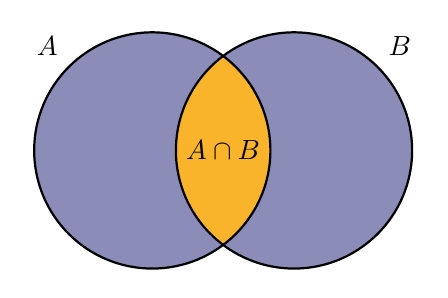
\begin{tikzpicture}[thick, set/.style = {circle, minimum size = 3cm, fill=MidnightBlue!50}]
		\node[set,label={135:$A$}] (A) at (0,0) {};
		\node[set,label={45:$B$}] (B) at (1.8,0) {};

		\begin{scope}
			\clip (0,0) circle(1.5cm);
			\clip (1.8,0) circle(1.5cm);
			\fill[Dandelion](0,0) circle(1.5cm);
		\end{scope}

		\draw (0,0) circle(1.5cm);
		\draw (1.8,0) circle(1.5cm);
		\node at (0.9,0) {$ A \cap B $};
	\end{tikzpicture}
	\caption{交集}
\end{figure}

如果两个集合没有公共元素,那么它们的交集为空集。\\

\subsection{并集(Union)}

假设$ A $和$ B $是两个集合,由它们所有元素合并在一起组成的集合,称为$ A $与$ B $的并集,表示为$ A \cup B $。

\begin{figure}[H]
	\centering
	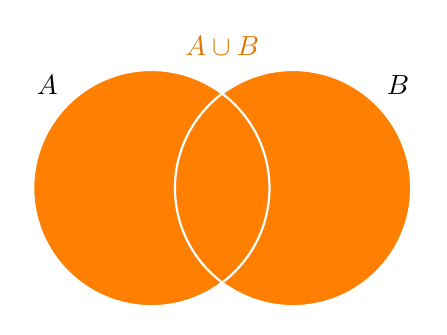
\begin{tikzpicture}
		\node [circle, fill=orange, minimum size=3cm, label={135:$A$}] (A) at (0,0){};
		\node [circle,
			fill=orange,
			minimum size =3cm,
			label={45:$B$}] (B) at (1.8,0){};

		\draw[white,thick] (0,0) circle(1.5cm);
		\draw[white,thick] (1.8,0) circle(1.5cm);
		\node[orange!90!black] at (0.9,1.8) {$ A \cup B $};
	\end{tikzpicture}
	\caption{并集}
\end{figure}

\vspace{0.5cm}

\subsection{差集(Difference)}

假设$ A $和$ B $是两个集合,由属于$ A $而不属于$ B $的元素组成的集合,称为$ A $与$ B $的差集,表示为$ A - B $。\\

差集运算不满足交换律,即$ A - B \neq B - A $。

\begin{figure}[H]
	\centering
	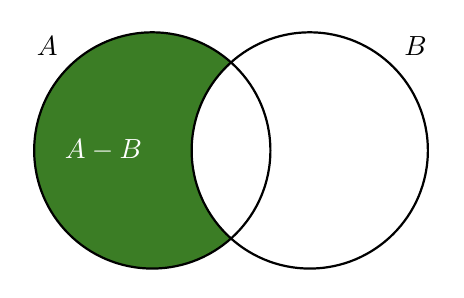
\begin{tikzpicture}[thick, set/.style = { circle, minimum size = 3cm}]
		\node[set,fill=OliveGreen,label={135:$A$}] (A) at (0,0) {};
		\node[set,fill=white,label={45:$B$}] (B) at (0:2) {};

		\draw (0,0) circle(1.5cm);
		\draw (2,0) circle(1.5cm);
		\node[left,white] at (A.center){$ A - B $};
	\end{tikzpicture}
	\caption{差集$ A - B $}
\end{figure}

\begin{figure}[H]
	\centering
	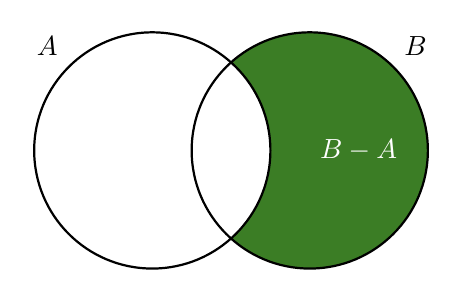
\begin{tikzpicture}[thick, set/.style = { circle, minimum size = 3cm}]
		\node[set,fill=OliveGreen,label={45:$B$}] (B) at (0:2) {};
		\node[set,fill=white,label={135:$A$}] (A) at (0,0) {};

		\draw (0,0) circle(1.5cm);
		\draw (2,0) circle(1.5cm);

		\node[right,white] at (B.center){$ B - A $};
	\end{tikzpicture}
	\caption{差集$ B - A $}
\end{figure}

\newpage

\section{集合恒等式}

\subsection{集合恒等式}

集合恒等式可以直接由对应的逻辑等价式证明。

\begin{tcolorbox}
	\mybox{幂等律 Idempotent Laws}
	\begin{align}
		A \cap A = A \\
		A \cup A = A
	\end{align}
\end{tcolorbox}

\begin{tcolorbox}
	\mybox{恒等律 Identity Laws}
	\begin{align}
		A \cap U = A \\
		A \cup \emptyset = A
	\end{align}
\end{tcolorbox}

\begin{tcolorbox}
	\mybox{支配律 Domination Laws}
	\begin{align}
		A \cap \emptyset = \emptyset \\
		A \cup U = U
	\end{align}
\end{tcolorbox}

\begin{tcolorbox}
	\mybox{双非律 Double Negation Law}
	\begin{align}
		\overline {\overline A} = A
	\end{align}
\end{tcolorbox}

\begin{tcolorbox}
	\mybox{交换律 Commutative Laws}
	\begin{align}
		A \cap B = B \cap A \\
		A \cup B = B \cup A
	\end{align}
\end{tcolorbox}

\begin{tcolorbox}
	\mybox{结合律 Associative Laws}
	\begin{align}
		(A \cap B) \cap C = A \cap (B \cap C) \\
		(A \cup B) \cup C = A \cup (B \cup C)
	\end{align}
\end{tcolorbox}

\begin{tcolorbox}
	\mybox{分配律 Distributive Laws}
	\begin{align}
		A \cap (B \cup C) = (A \cap B) \cup (A \cap C) \\
		A \cup (B \cap C) = (A \cup B) \cap (A \cup C)
	\end{align}
\end{tcolorbox}

\begin{tcolorbox}
	\mybox{德摩根律 De Morgan's Laws}
	\begin{align}
		\overline{A \cap B} = \overline A \cup \overline B
	\end{align}
\end{tcolorbox}

\begin{tcolorbox}
	\mybox{吸收律 Absorption Laws}
	\begin{align}
		A \cap (A \cup B) = A \\
		A \cup (A \cap B) = A
	\end{align}
\end{tcolorbox}

\begin{tcolorbox}
	\mybox{证明}
	$ \overline{A \cup (B \cap C)} = (\overline C \cup \overline B) \cap \overline A $
	\begin{align*}
		 & \overline{A \cup (B \cap C)}                      \\
		 & = \overline A \cap \overline{B \cap C}            \\
		 & = \overline A \cap (\overline B \cup \overline C) \\
		 & = (\overline B \cup \overline C) \cap \overline A \\
		 & = (\overline C \cup \overline B) \cap \overline A
	\end{align*}
\end{tcolorbox}

\begin{tcolorbox}
	\mybox{Exercise}
	一共有40个学生,有3门课程可供学生选择(C语言、离散数学、软件工程)。\\
	7人没有选任何课程;\\
	16人选软件工程;\\
	10人选C语言;\\
	5人同时选离散数学和软件工程;\\
	4人同时选离散数学和C语言;\\
	3人同时选软件工程和C语言;\\
	2人同时选离散数学、软件工程和C语言。\\

	\begin{figure}[H]
		\centering
		\begin{tikzpicture}
			\tikzset{venn circle/.style={draw,circle,minimum width=6cm,fill=#1,opacity=0.4}}
			\node [] () at (-2, -3) {C语言};
			\node [] () at (2, 7) {离散数学};
			\node [] () at (6, -3) {软件工程};
			\node [] () at (6, 7) {$ U $};
			\node [] () at (6, 6.5) {7};
			\node [venn circle = red] (A) at (0,0) {5};
			\node [venn circle = blue] (B) at (60:4cm) {10};
			\node [venn circle = green] (C) at (0:4cm) {10};
			\node[left] at (barycentric cs:A=1/2,B=1/2) {2};
			\node[below] at (barycentric cs:A=1/2,C=1/2) {1};
			\node[right] at (barycentric cs:B=1/2,C=1/2) {3};
			\node[below] at (barycentric cs:A=1/3,B=1/3,C=1/3) {2};
		\end{tikzpicture}
	\end{figure}
\end{tcolorbox}

\newpage

\section{笛卡尔积}

\subsection{元组(Tuple)}

有时候元素聚集中次序是很重要的,由于集合是无序的,所以就需要一种不同的结构表示有序的聚集,这就是有序$ n $元组(ordered-n-tuple)。\\

有序$ n $元组$ (a_1,\ a_2,\ \dots,\ a_n) $是以$ a_1 $为第$ 1 $个元素,$ a_2 $为第$ 2 $个元素,$ a_n $为第$ n $个元素的有序聚集。\\

只有两个有序$ n $元组的每一对对应的元素都相等,那么这两个有序$ n $元组是相等的,即:

\vspace{-0.5cm}

$$
	(a_1,\ a_2,\ \dots,\ a_n) = (b_1,\ b_2,\ \dots,\ b_n)\ \text{iff}\ i = 1,\ 2,\ \dots,\ n
$$

需要注意,$ (a,\ b) $与$ (b,\ a) $不相等,除非$ a = b $。\\

\subsection{笛卡尔积(Cartesian Product)}

假设有两个集合$ A $和$ B $,$ A $和$ B $的笛卡尔积用$ A \times B $表示,笛卡尔积是所有序偶$ (a,\ b) $的集合,其中$ a \in A $且$ b \in B $。

\vspace{-0.5cm}

$$
	A \times B = \{(a,\ b)\ |\ a \in A \wedge b \in B\}
$$

笛卡尔积$ A \times B $和$ B \times A $是不相等的,除非$ A = \emptyset $或$ B = \emptyset $或$ A = B $。

\begin{tcolorbox}
	\mybox{Exercise}
	笛卡尔积\\
	学生集合$ S = \{s1,\ s2\} $\\
	课程集合$ C = \{c1,\ c2,\ c3\} $\\
	$ S \times C = \{(s1,\ c1),\ (s1,\ c2),\ (s1,\ c3),\ (s2,\ c1),\ (s2,\ c2),\ (s2,\ c3)\} $\\
	笛卡尔积$ S \times C $表示学生选课的所有可能情况\\
\end{tcolorbox}

\begin{tcolorbox}
	\mybox{Exercise}
	笛卡尔积$ A \times B \times C $\\
	$ A = \{0,\ 1\} $\\
	$ B = \{1,\ 2\} $\\
	$ C = \{0,\ 1,\ 2\} $
	\begin{align*}
		A \times B \times C = \{(0, 1, 0), (0, 1, 1), (0, 1, 2), (0, 2, 0), (0, 2, 1), (0, 2, 2), \\
		(1, 1, 0), (1, 1, 1), (1, 1, 2), (1, 2, 0), (1, 2, 1), (1, 2, 2)\}
	\end{align*}
\end{tcolorbox}

一个集合与自身的笛卡尔积,如$ A \times A $可表示为$ A^2 $。

\begin{tcolorbox}
	\mybox{Exercise}
	笛卡尔积$ A^2 $\\
	$ A = \{1,\ 2\} $\\
	$ A^2 = \{(1,\ 1),\ (1,\ 2),\ (2,\ 1),\ (2,\ 2)\} $
\end{tcolorbox}

\newpage